\documentclass{article}
\usepackage{listings}
\usepackage{xcolor}
\usepackage{graphicx}


\title{ACN LAB - 01 \\Socket Programming for Client-Server Communication Using Python}
\author{Chaitanya Talware (MIS No: 712422005) \\ Yogesh Toshniwal (MIS No: 712422021)}

\date{}

\lstdefinestyle{python}{
    language=Python,
    basicstyle=\ttfamily\small,
    numbers=left,
    numberstyle=\tiny\color{gray},
    stepnumber=1,
    numbersep=5pt,
    backgroundcolor=\color{lightgray},
    showstringspaces=false,
    frame=single,
    rulecolor=\color{black},
    breaklines=true,
    breakatwhitespace=true,
    keywordstyle=\color{blue}\bfseries,
    commentstyle=\color{green},
    stringstyle=\color{red},
}

\begin{document}

\maketitle
\section{Introduction}
Socket programming enables communication between programs over a network using the client-server model. In this assignment, we implement a client-server system using Python's socket module. The server listens for client requests and provides mathematical operations such as square, square root, and factorial. The client sends a request with the operation and number, and the server computes and returns the result.

The available operations are:
\begin{itemize}
    \item \texttt{sqrt}: Calculate the square root of a number.
    \item \texttt{square}: Calculate the square of a number.
    \item \texttt{factorial}: Calculate the factorial of a number.
\end{itemize}

\section{Source Code }
\subsection{Client Code}
\begin{lstlisting}[style=python]
import socket

def main():
    client_socket = socket.socket(socket.AF_INET, socket.SOCK_STREAM)
    host = 'localhost'
    port = 12346
    client_socket.connect((host, port))

    print("Available operations: 'sqrt', 'square', 'factorial' (or 1, 2, 3)")
    print("Enter 'q' to quit.")

    while True:
        operation = input("Enter the operation you want to perform (q to quit): ")
        
        if operation == 'q':
            client_socket.send(b'q')  # Send quit command to server
            print('Exiting...')
            break

        number = int(input("Enter the number: "))
        data = "{} {}".format(operation, number)
        client_socket.send(data.encode('utf-8'))

        result = client_socket.recv(1024).decode('utf-8')
        print("Result: {}".format(result))

    client_socket.close()

if __name__ == "__main__":
    main()
\end{lstlisting}

\subsection{Server Code}
\begin{lstlisting}[style=python]
import socket
import math

def calculate_sqrt(number):
    return math.sqrt(number)

def calculate_square(number):
    return number ** 2

def calculate_factorial(number):
    if number == 0:
        return 1
    return number * calculate_factorial(number - 1)

def main():
    server_socket = socket.socket(socket.AF_INET, socket.SOCK_STREAM)
    host = '0.0.0.0'
    port = 12346
    server_socket.bind((host, port))

    server_socket.listen(5)
    print("Server is listening on {}:{}".format(host, port))

    while True:
        client_socket, addr = server_socket.accept()
        print("Accepted connection from {}:{}".format(addr[0], addr[1]))

        while True:
            data = client_socket.recv(1024).decode('utf-8')
            if data == 'q':  
                print("Client {}:{} disconnected.".format(addr[0], addr[1]))
                break  

            if data == '':
                print("Disconnected - from {}:{}".format(addr[0], addr[1]))
                break
            
            operation, number = data.split()
            number = float(number)

            if operation == 'sqrt' or operation == '1':
                result = calculate_sqrt(number)
            elif operation == 'square' or operation == '2':
                result = calculate_square(number)
            elif operation == 'factorial' or operation == '3':
                result = calculate_factorial(int(number))
            else:
                result = "Invalid operation"

            client_socket.send(str(result).encode('utf-8'))

        client_socket.close()  # Close the client socket after exiting the loop

        \section{Output}
        \subsection{Server Output}
        \subsection{Client Output}
if __name__ == "__main__":
    main()
\end{lstlisting}
\section{Output}
\subsection{Server Output}
\centering
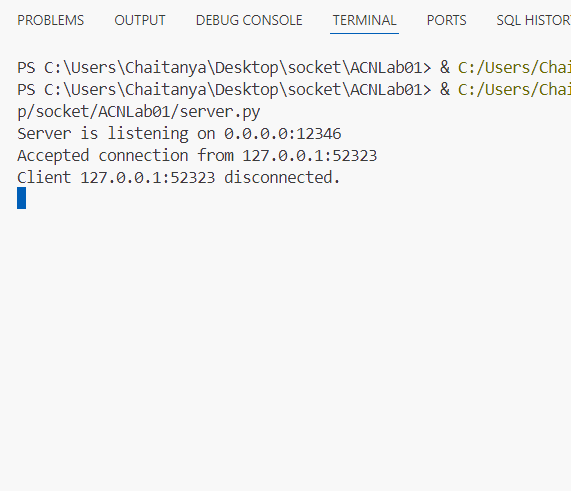
\includegraphics{server.png}
\subsection{Client Output}
\centering
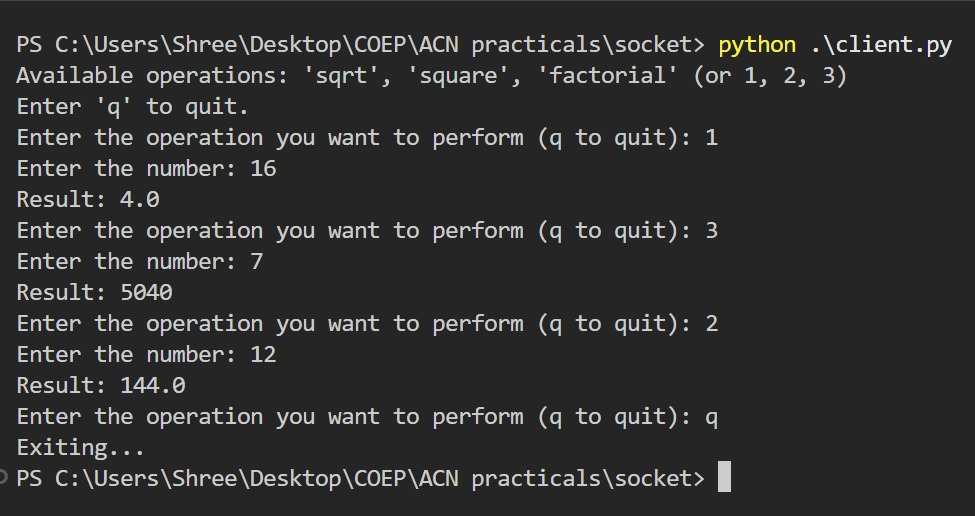
\includegraphics[width = 15cm]{client.jpeg}
\subsection{Wireshark Output}
\centering
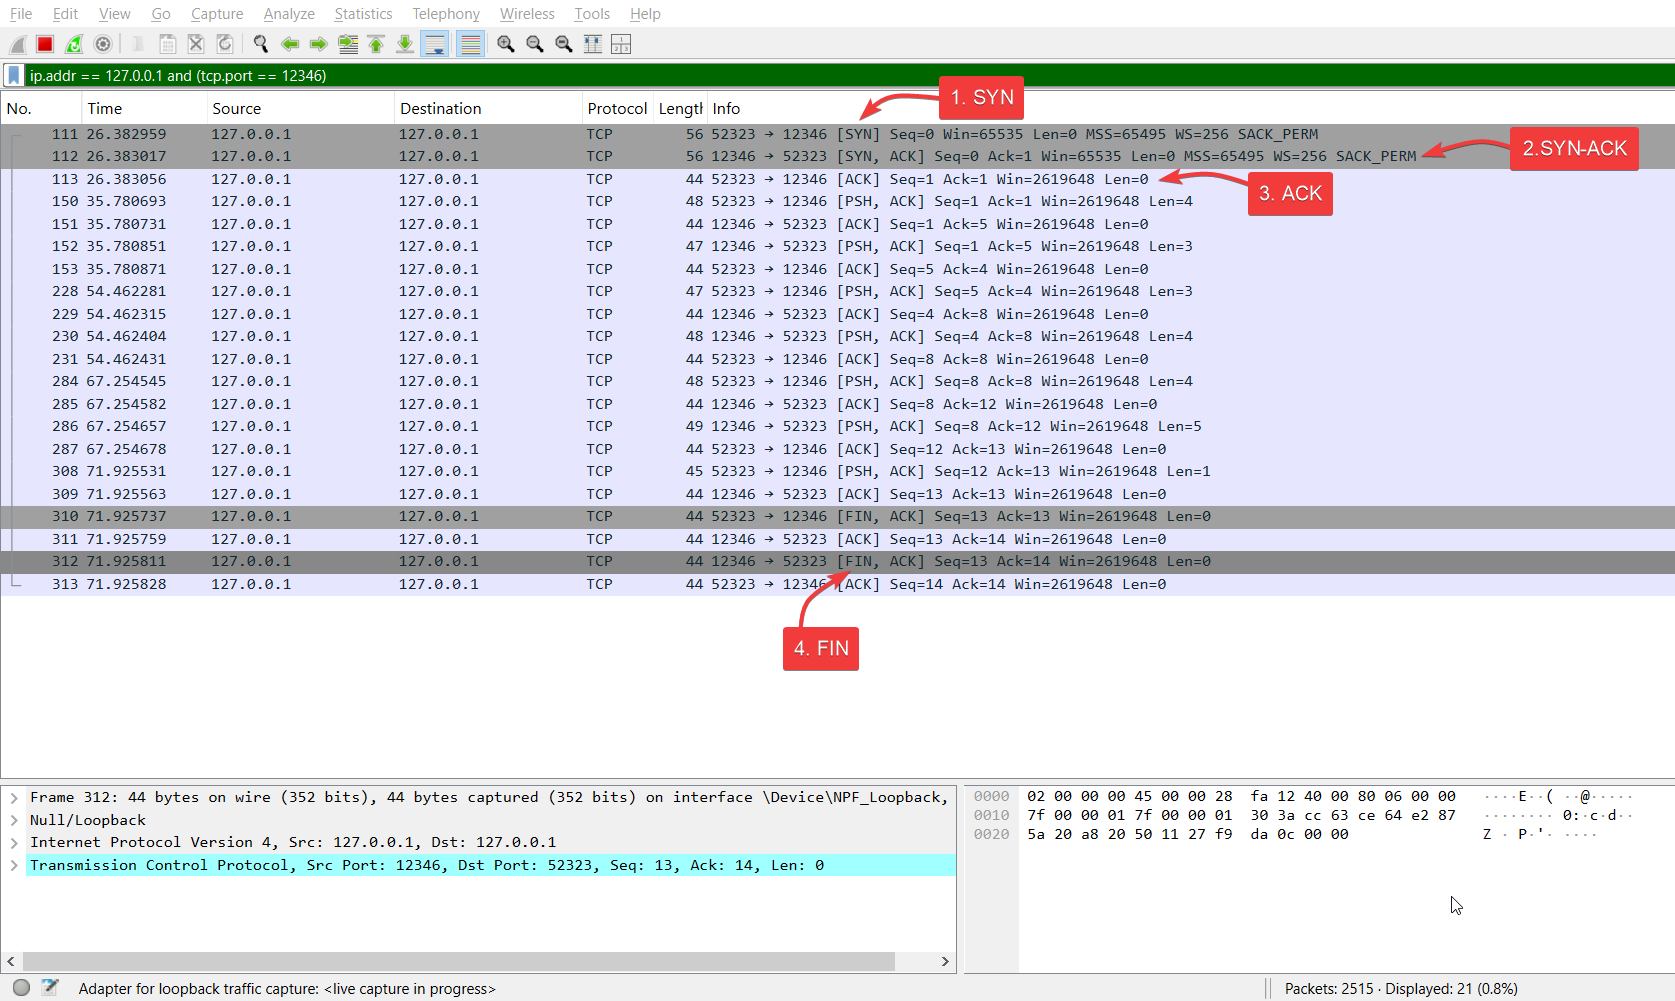
\includegraphics[angle=270, width=\textwidth]{wireshark.png}


\end{document}
